% !TEX encoding = UTF-8
% !TEX program = pdflatex
% !TEX spellcheck = es_ES

\documentclass[spanish,a4paper]{europasscv}
\usepackage[spanish]{babel}
\usepackage{pdfpages}

\ecvname{Salvador Martin}
\ecvaddress{Via Antrodoco 1, 67100, AQ (Italy)}
\ecvmobile{+39 380 193 1121}
%\ecvtelephone{+353 127 6689}
%\ecvworkphone{+353 999 888 777}
\ecvemail{salvador.martin.cu@gmail.com}
%\ecvhomepage{www.myhomepage.com www.another-homepage.com}
% \ecvgithubpage{www.github.com/smith}
\ecvlinkedinpage{www.linkedin.com/in/salvador-martin}
%\ecvim{AOL Messenger}{katie.smith}
%\ecvim{Google Talk}{ksmith}
\ecvim{Skype}{salva2015cu}

\ecvdateofbirth{20 Gennaio 1983}
\ecvnationality{Cubano}
\ecvgender{Maschile}

\ecvpicture[width=2.8cm]{yo}

\date{}

\begin{document}
  \begin{europasscv}

  \ecvpersonalinfo

% \ecvbigitem{Job applied for}{European project manager}

  \ecvsection{ExPERIENcia PROFESIONAL}
  \ecvtitle{Sep, 2011 -- Sep, 2015}{Profesor}
  \ecvitem{}{Universidad de Matanzas ''Camilo Cienfuegos'', Matanzas (Cuba)}
  \ecvitem{Profesor Asistente,\qquad \qquad \qquad \qquad Sep, 2013 -- Sep, 2015}{
  	\begin{ecvitemize}
  		\item Preparaci\'on metodol\'ogica y realizaci\'on, en colaboraci\'on con el profesor principal, de la asignatura Termodin\'amica T\'ecnica 1 y 2, al tercer año de la carrera de Ingenier\'ia Mec\'anica,
  		\item Profesor de la asignatura optativa Principios de la Energ\'ia Renovable en la carrera de Ingenier\'ia Mec\'anica,
  		\item Colaboraci\'on con la carrera Ingenier\'ia Civil, impartiendo la asignatura optativa Bases de Energ\'ias Renovables,
  		\item Colaboraci\'on con la carrera Ingenier\'ia Industrial, impartiendo la asignatura Procesos Tecnol\'ogicos.
  	\end{ecvitemize}
  }  
  \ecvitem{Profesor Instructor, \qquad \qquad \qquad Sep, 2012 -- Sep, 2013}{
  	Inicio y finalizaci\'on con \'exito en la preparaci\'on como profesor universitario, teniendo como tarea principal la preparaci\'on metodol\'ogica y realizaci\'on de la asignatura Termodin\'amica T\'ecnica 1 y 2, al tercer año de la carrera de Ingenier\'ia Mec\'anica.
  }
  \ecvitem{Profesor Asociado \qquad \qquad \qquad \qquad  Sep, 2011 -- Sep, 2012}{
  	Profesor de la asignatura de Sistemas de Informaci\'on en la carrera Contabilidad y Finanzas. El objetivo principal de esta asignatura es proporcionar los conocimientos b\'asicos sobre la codificaci\'on correcta y el cifrado inform\'atico de la informaci\'on contable, as\'i como las herramientas y t\'ecnicas para su implementaci\'on.
  }  
  \ecvitem{Actividades generales}{
  	\begin{ecvitemize}
  		\item Dirigir, tutorear y seguir la investigaci\'on de estudiantes en temas relevantes, acorde con las l\'ineas de investigaci\'on de la facultad de Ingenier\'ia Mec\'anica.
  		\item Preparar, dise\~nar, dirigir y$/$o presentar oryectos de investigaci\'on al consejo cient\'ifico de la facultad de Ingenier\'ia Mec\'anica.
  		\item Organizar y desarrollar trabajo de campo con los estudiantes en las industrias del territorio, con el objetivo de desarrollar v\'inculos de trabajo y habilidades ''en caliente'' con la solucion de tareas tecnol\'gicas asignadas.
  		\item Participar en sesiones de tesis como jurado, oponente o tutor/co--tutor. 
  	\end{ecvitemize}
  }
  \ecvtitle{Dic, 2013 -- Sep, 2015}{Administrador de Red Inform\'atica}
  \ecvitem{}{Universidad de Matanzas ''Camilo Cienfuegos'', Matanzas (Cuba)}
  \ecvitem{}{
  	\begin{ecvitemize}
  		\item Desarrollo, diseño, optimizaci\'on y mantenimiento de la red inform\'atica de la universidad,
  		\item Configuraci\'on y mantenimiento de conmutadores, enrutadores y equipos de comunicaci\'on,
  		\item Optimizaci\'on y mantenimiento de servicios de red inform\'atica (DNS, DHCP, servidor web (IIS, Apache), proxy de red (IPTables, servidor ISA, Squeeze), Active Directory (Linux y Windows), servicio de correo electr\'onico),
  		\item Instalaci\'on, configuraci\'on y mantenimiento de servidores dedicados en distribuci\'on de Windows o Linux (f\'isicos$/$Cloud),
  		\item Instalaci\'on, configuraci\'on y mantenimiento de estaciones de trabajo dedicadas a servicios universitarios.
  	\end{ecvitemize}
  }
  \pagebreak
  \ecvtitle{Mar 2007 -- Sep 2011}{Especialista en Seguridad de Redes Infrom\'aticas}
  \ecvitem{}{Servicios Especializados en Protecci\'on S.A. (Cuba)}
  \ecvitem{}{Ejecuci\'on de estudios detallados y evaluaci\'on del flujo de informaci\'on, an\'alisis de trazas y detecci\'on de fallas y vulnerabilidades de seguridad en redes inform\'aticas. Desarrollo de diagn\'osticos (GFI Languard, Tenable Nessus), as\'i como el redise\~no de redes infrom\'aticas con la implementaci\'on de sistemas de detecci\'on de intrusos (IDS) y protecci\'on contra ciberataques desde$/$hacia la red de TI local a empresas de terceros.
  }
 \ecvsection{InSTRUcci\'on y FORMAcI\'ON}
  \ecvtitlelevel{Sep 2015 -- Now}{PhD (ongoing)}{}
  \ecvitem{\textbf{T\'itulo de la Tesis}}{Smart grids: Fault and attack detection, and robust control design.}
  \ecvitem{\textbf{Director}}{Stefano Di Gennaro}
  \ecvitem{}{Università degli Studi dell'Aquila, L'Aquila (Italy)}
  \ecvtitlelevel{2004 -- 2009}{Ingeniero Mec\'anico}{}
  \ecvitem{\textbf{T\'itulo de la Tesis}}{Propuesta de un sistema fotovoltaico para el suministro de electricidad a los principales consumidores de la rector\'ia de la Universidad de Matanzas ''Camilo Cienfuegos''}
  \ecvitem{\textbf{Director}}{Ju\'an I. V\'eliz Alonso}
  \ecvitem{}{Universidad de Matanzas ''Camilo Cienfuegos'', Matanzas (Cuba)}
  
  \ecvsection{Competencias personales}
  \ecvmothertongue{Espa\~nol}
  \ecvlanguageheader
  \ecvlanguage{Ingl\'es}{B1}{B2}{B2}{B1}{B1}
  \ecvlastlanguage{Italiano}{B2}{B2}{B2}{B1}{B1}
  \ecvlanguagefooter
    
  \ecvblueitem{Competencias comunicativas}{
  \begin{ecvitemize}
  	\item Formo parte del grupo de voluntarios en Erasmus Students Network (ESN) - Aquilasmus que ayuda a los nuevos estudiantes Erasmus, promoviendo y organizando, como parte del equipo, varias actividades extracurriculares,
  	\item Durante mi investigaci\'on de doctorado, trabaj\'e y colabor\'e con otros aspirantes al grado de doctor de diferentes campos.
  \end{ecvitemize}
  }
  
  \ecvblueitem{Competencias organizacionales$/$gesti\'on}{
  \begin{ecvitemize}
    \item Mientras trabajaba como profesor en la Universidad de Matanzas ''Camilo Cienfuegos'', estaba a cargo de la gesti\'on y organizaci\'on de actividades con los estudiantes, dentro y fuera del aula,
    \item Gesti\'on y organizaci\'on de proyectos de investigaci\'on y gesti\'on de tesis de estudiantes.
    \item Mientras trabajaba como Especialista en Seguridad de Redes Infrom\'aticas, estaba a cargo de hacer presentaciones con los ejecutivos de las empresas que contrataron mis servicios, donde se brindaban consejos sobre buenas pr\'acticas en el uso de las TIC, adem\'as de la gesti\'on comercial y promoci\'on del servicio.
  \end{ecvitemize}
  }

  %\ecvdigitalcompetence{\ecvBasic}{\ecvIndependent}{\ecvProficient}{\ecvIndependent}{\ecvBasic}
  
  \ecvblueitem{Competencias digitales}{\textbf{Uso general}}{}
  	\ecvitem{}{Microsoft Office, Open Office, Libre Office}{}
  \ecvitem{}{\textbf{Sistemas Operativos}}{}
  	\ecvitem{}{Microsoft Windows, Linux (Debian, Ubuntu, SUSE)}{}
  \ecvitem{}{\textbf{Dise\~no}}{}
  	\ecvitem{}{AutoCAD, Mechanical Desktop, Adobe Fireworks, TKSolver}{}
  \ecvitem{}{\textbf{Programaci\'on y simulaci\'on}}{}
  	\ecvitem{}{Matlab, Simulink, Latex, TKSolver, HTML, PHP}{}
  \ecvitem{}{\textbf{Administraci\'on de redes inform\'aticas}}{}
  	\ecvitem{}{DNS, DHCP, Web Servers (IIS, Apache), Network Proxy (IPTables, ISA Server, Squeeze), Active Directory (Linux and Windows), e--mail Service, Virtual Machines (VM Ware, VirtualBox)}{}
    
  \ecvblueitem{Otras competencias}{
  	En mi tiempo libre me gusta leer un buen libro, encontrarme y compartir con mis amigos y pasar tiempo con ellos bailando, cantando, escuchando buena m\'usica: salsa, merengue, bachata, viejos cl\'asicos, blues, R \& B, Jazz. Me apasiona la pr\'actica de deportes: nadar, entrenar artes marciales, baseball y cualquier juego en general.
  }

  \ecvblueitem{Permiso de conducir}{A, B}
  
  \ecvsection{Otras infromaciones}
  \ecvbigitem{Corsi avanzati}{}
  \ecvtitle{2017}{Formal Methods for the Control of Large-scale Networked Nonlinear Systems with Logic Specifications}
  \ecvitem{}{by Alessandro Borri, Maria Domenica Di Benedetto, Giordano Pola and Pierdomenico Pepe}
  \ecvitem{}{Università degli Studi dell'Aquila, L'Aquila (Italy)}
  \ecvtitle{}{7th oCPS PhD School on Cyber-Physical Systems}
  \ecvitem{}{IMT School for Advanced Studies, Lucca (Italy)}
  \ecvtitle{}{Energy-based modeling and control of physical system}
  \ecvitem{}{by Arjan van der Schaft (University of Groningen) and Dimitri Jeltsema (TU Delft (Netherland))}
  \ecvitem{}{CentraleSup\'elec, Paris (France)}
  \ecvtitle{2016}{Tools for nonlinear control, Lyapunov function, positivity, applications}
  \ecvitem{}{by Fr\'ed\'eric Mazenc (CentraleSup\'elec (France))}
  \ecvitem{}{Università degli Studi dell'Aquila, L'Aquila (Italy)}
  \ecvtitle{}{Cyber-Physical systems control: Algebraic and Optimization techniques}
  \ecvitem{}{by Raphaël Jungers (UCL (Belgium))}
  \ecvitem{}{Università degli Studi dell'Aquila, L'Aquila (Italy)}
  
  %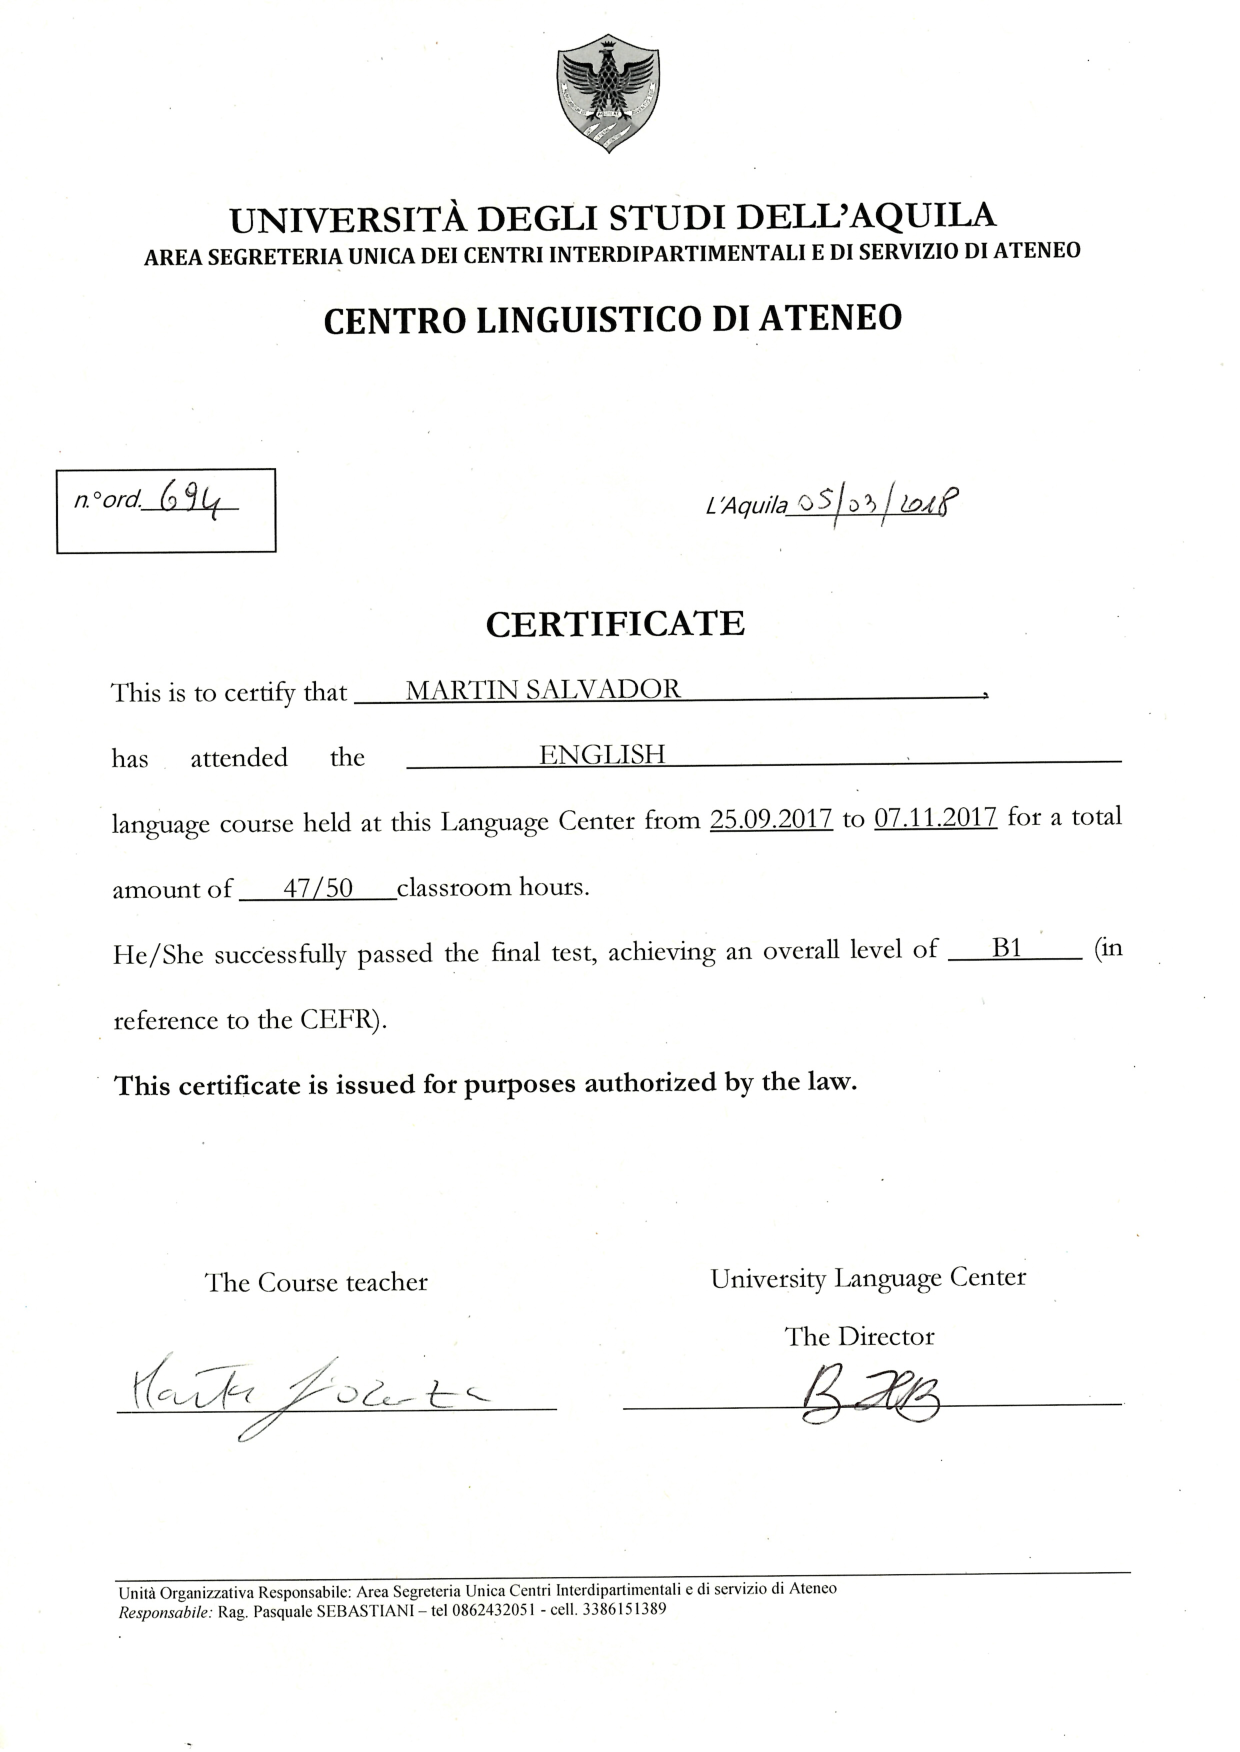
\includepdf{English(en)}
  %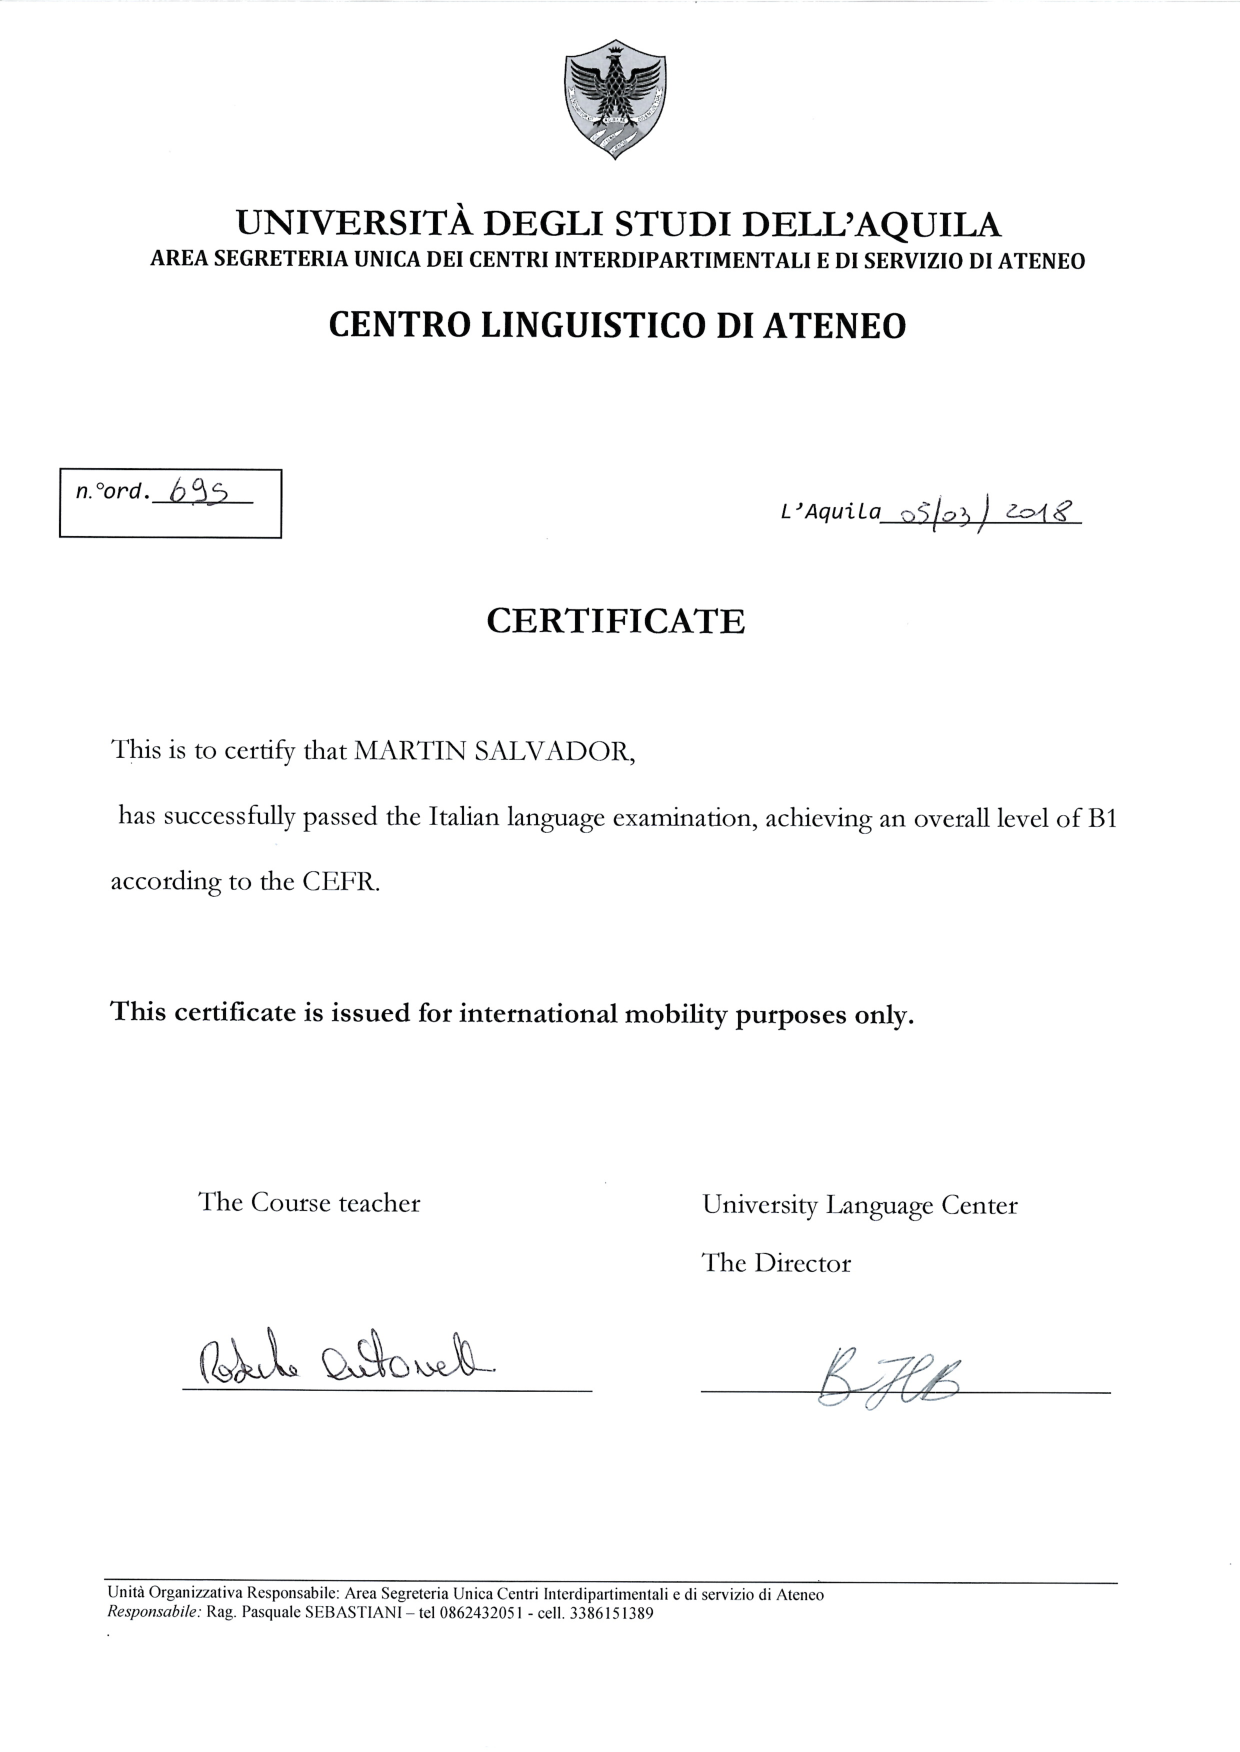
\includepdf{Italian(en)}
  \end{europasscv}

\end{document}